\documentclass[aspectratio=169,professionalfonts]{beamer}
\usetheme{Madrid}
\usecolortheme{dolphin}
\usefonttheme{professionalfonts}
\setbeamertemplate{navigation symbols}{}
\setbeamertemplate{footline}[frame number]

\usepackage[utf8]{inputenc}
\usepackage[T1]{fontenc}
\usepackage{lmodern}
\usepackage{amsmath,amssymb,mathtools}
\usepackage{booktabs}
\usepackage{tikz}
\usetikzlibrary{positioning,arrows.meta}
\usepackage{xcolor}
\usepackage{hyperref}
\usepackage{enumitem}

\definecolor{DeepBlue}{RGB}{20,52,102}
\definecolor{SoftBlue}{RGB}{64,114,176}
\definecolor{AccentOrange}{RGB}{217,114,31}
\definecolor{LightGray}{RGB}{245,247,250}

\setbeamercolor{title}{fg=DeepBlue}
\setbeamercolor{frametitle}{fg=DeepBlue}
\setbeamercolor{structure}{fg=SoftBlue}
\setbeamercolor{block title}{bg=DeepBlue!10,fg=DeepBlue}
\setbeamercolor{block body}{bg=LightGray,fg=black}
\setbeamercolor{alerted text}{fg=AccentOrange}

\title{LLM Matrix Inversion}
\subtitle{LLM Architecture, Training, and Evaluation for Structured Numeric Generation}
\author{Pranav Tikkawar}
\date{May 04, 2026}

\begin{document}

\begin{frame}
  \titlepage
\end{frame}

\begin{frame}{What this project is}
\begin{block}{Goal}
Given a text description of a real-valued matrix $A$, the model should output a strictly formatted text block containing a numerically correct inverse $A^{-1}$.
\end{block}

\vspace{0.5em}
\begin{itemize}[itemsep=0.6em]
    \item This is a \alert{dual objective}: formatting must be parseable since LLMs are prone to generating text that looks reasonable but is not actually correct, and the numbers must actually invert the matrix instead of providing a trivial solution via some pattern.
    \item A prediction only counts as good if it survives both checks.
    \item Typical failures: looping text, parseable but wrong numbers, and outputs that resemble $A$ or $-A$ rather than $A^{-1}$.
\end{itemize}
\end{frame}

\begin{frame}{3 methods for getting better LLM results}
\begin{columns}[T,totalwidth=\textwidth]
\column{0.32\textwidth}
\begin{block}{Initial Promping}
Initial prompting is the most basic method: just give the model a clear instruction and hope for the best. This can work for simple tasks, but for complex tasks, it often leads to poor performance.
\end{block} 
\column{0.32\textwidth}
\begin{block}{LoRA fine-tuning}
LoRA fine-tuning allows us to adapt the model's weights to our specific task without needing to update the entire model, which can be more efficient and effective for specialized tasks.
\end{block}
\column{0.32\textwidth}
\begin{block}{Multi-shot prompting}
Multi-shot prompting provides the model with several examples of the desired output format and content, which can help it learn the pattern and improve its performance on the task.
\end{block}
\end{columns}

\vspace{0.8em}
I predominantly used a mix of LoRA fine-tuning and multi-shot prompting, since initial prompting alone was not sufficient to achieve good results on the matrix inversion task.
    
\end{frame}

\begin{frame}{Overarching architecture}
\centering
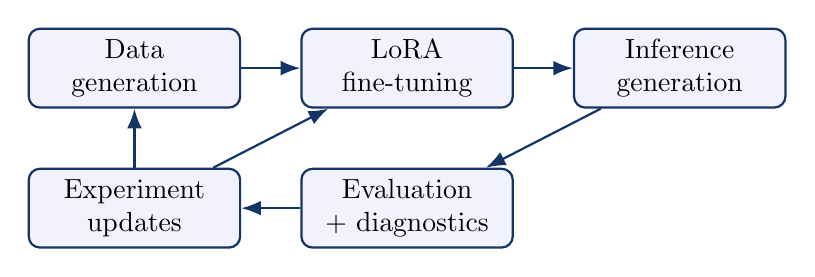
\begin{tikzpicture}[
    node distance=0.75cm and 0.75cm,
    box/.style={draw=DeepBlue, rounded corners, thick, align=center, minimum height=1.0cm, fill=blue!5, text width=2.45cm},
    arrow/.style={-{Latex[length=2.5mm]}, thick, DeepBlue}
]
\node[box] (gen) {Data\\generation};
\node[box, right=of gen] (train) {LoRA\\fine-tuning};
\node[box, right=of train] (infer) {Inference\\generation};
\node[box, below=of train] (eval) {Evaluation\\+ diagnostics};
\node[box, left=of eval] (agent) {Experiment\\updates};
\draw[arrow] (gen) -- (train);
\draw[arrow] (train) -- (infer);
\draw[arrow] (infer) -- (eval);
\draw[arrow] (eval) -- (agent);
\draw[arrow] (agent) -- (gen);
\draw[arrow] (agent) -- (train);
\end{tikzpicture}

\vspace{0.8em}
\begin{itemize}[itemsep=0.5em]
    \item The point is rapid iteration: generate data, fine-tune adapters, evaluate, inspect failures, and change the next run.
    \item The diagnostics are designed to tell whether the main problem is formatting, optimization, or numeric behavior.
\end{itemize}
\end{frame}

\begin{frame}{Why LoRA and how it links to stochastics}
\begin{block}{LoRA idea}
Freeze a pretrained weight matrix $W$ and learn a low-rank update
\[
W' = W + BA,
\]
with small rank, instead of updating all weights.
\end{block}

\begin{itemize}[itemsep=0.6em]
    \item LoRA reduces trainable parameters and memory by learning low-rank adapter matrices rather than fully updating pretrained weights \cite{lora}.
    \item Training is still stochastic optimization: mini-batches produce noisy gradient estimates, but those updates now live in a constrained low-rank subspace \cite{peft}.
    \item For this project, that means a key question is whether the adapter has enough capacity to learn both strict syntax and precise numerics.
\end{itemize}
\end{frame}

\begin{frame}{How I judge success}
\begin{block}{Primary metric}
Use the inversion residual
\[
\|A\hat{X} - I\|_F
\]
as the main score.
\end{block}

\begin{itemize}[itemsep=0.6em]
    \item Near zero means the output behaves like an inverse.
    \item Large values indicate that even a well-formatted answer is numerically wrong.
    \item I also track parse success, stop reason, token count, right residual $\|\hat{X}A-I\|_F$, and whether $\hat{X}$ is closer to $A$ or $-A$ than to $A^{-1}$.
\end{itemize}
\end{frame}

\begin{frame}{Three output categories}

    
Most of the outputs I get fall into one of three categories: 

\begin{columns}[T,totalwidth=\textwidth]

\column{0.32\textwidth}
\begin{block}{No output / unreadable}
\begin{itemize}[itemsep=0.45em]
  \item Looping or truncated generations.
  \item Multiple \texttt{Inverse:} headers, extra text, or broken layout.
  \item Parser fails, so we cannot even compute $A\hat{X}$ or residuals.
\end{itemize}
\end{block}

\column{0.32\textwidth}
\begin{block}{Looks like $-A$}
\begin{itemize}[itemsep=0.45em]
  \item Output is a clean matrix but entries are roughly the negative of $A$.
  \item $\|\hat{X}+A\|_F$ is smaller than $\|\hat{X}-A^{-1}\|_F$.
  \item $ \|A\hat{X}-I\|_F$ remains large, so this is not an inverse.
\end{itemize}
\end{block}

\column{0.32\textwidth}
\begin{block}{Looks like $1/A$ (elementwise inverse)}
\begin{itemize}[itemsep=0.45em]
  \item Clean, single matrix in the right format.
  \item Output is still incorrect as it resembles the elementwise inverse rather than the true matrix inverse.
\end{itemize}
\end{block}

\end{columns}

\vspace{0.8em}

Unfortunately, the model does not seem to ever produce a true inverse on the eval set, but it does produce outputs in the last two categories that are close enough to parse and evaluate, which gives us some signal to work with.

\end{frame}

\begin{frame}{Results and Potential Symptoms}
\begin{itemize}[itemsep=0.7em]
  \item The first output category (no output/unreadable) is the most common among the no-shot, pre-trained model, and nearly disappears with LoRA fine-tuning and multi-shot prompting, which suggests that the model is learning to follow the output format and stop appropriately.
  \item With low training and low data regimes, the second category (looks like $-A$) is more common, which could indicate that the model is picking up on some superficial pattern in the input matrix rather than learning the true mathematical relationship.
  \item The third category (looks like $1/A$) appears more frequently with multi-shot prompting, which might suggest that the model is learning to produce a matrix that is related to the input but is not actually the correct inverse, possibly due to overfitting to the examples provided in the prompt rather than generalizing the underlying mathematical concept.
\end{itemize}

\vspace{0.5em}

While the model never produces a correct inverse, the shift in output categories with different training methods provides insight into how the model is learning and where it might be going wrong, which can inform our next steps in improving its performance on this task.
\end{frame}

\begin{frame}{Next steps}
\begin{itemize}[itemsep=0.7em]
  \item \textbf{More data}: generate more and harder matrices to better
        cover the space the model needs to invert.
  \item \textbf{Better parsing}: tighten the output format and add
        guardrails so looping and extra text are less likely.
  \item \textbf{More multi-shot prompting}: show more varied correct
        inverses so the model sees the pattern clearly.
  \item \textbf{Longer, targeted training}: run longer LoRA training
        on curated hard examples once the basics look solid.
\end{itemize}
\end{frame}

\begin{frame}{Main message}
\begin{itemize}[itemsep=0.75em]
    \item The project is really about \alert{structured numeric generation}, not just text generation.
    \item LoRA makes the experimentation loop fast enough to test data, rank, decoding, and formatting hypotheses.
    \item The central empirical question is where the model fails first: parsing, looping, or true inversion quality.
\end{itemize}

\vspace{1em}
\centering
\Large Questions
\end{frame}

\begin{thebibliography}{9}
\bibitem{lora}
Edward J. Hu et al.
\newblock \emph{LoRA: Low-Rank Adaptation of Large Language Models}.
\newblock arXiv:2106.09685, 2021.

\bibitem{peft}
Hugging Face.
\newblock \emph{PEFT documentation: LoRA}.
\newblock \url{https://huggingface.co/docs/peft/v0.8.0/package_reference/lora}.
\end{thebibliography}

\end{document}